%% Supplementary Materials -- Genetics in Medicine (GIM) submission
%% Compile:  latexmk -pdf supplementary.tex
%% Source of truth for content: ../../supplementary/supplementary.md

\documentclass[12pt]{article}

\usepackage[a4paper,margin=2.5cm]{geometry}
\usepackage{amsmath}
\usepackage{amssymb}
\usepackage{booktabs}
\usepackage{graphicx}
\usepackage[hidelinks]{hyperref}

\graphicspath{{../../figures/}}
\emergencystretch=2em

%% S-prefixed numbering for supplementary display items
\renewcommand{\thefigure}{S\arabic{figure}}
\renewcommand{\thetable}{S\arabic{table}}

\title{Supplementary Materials\\[1ex]
\large for ``Marginal Contribution of Cross-Lingual Evidence Extraction to
ACMG/AMP Variant Classification: An Ablation Study of a Multi-Agent
Literature Curation System''}
\author{[Author list TBD]}
\date{}

\begin{document}

\maketitle

\noindent Data source: \path{docs/gim/supplementary/reports/} (committed
copy, mirrored from \path{benchmark/data/reports/nar_ablation/},
2026-08-12 runs).

\tableofcontents

\clearpage

\section*{Supplementary Figure S1: Evidence Items by ACMG Category}
\addcontentsline{toc}{section}{Supplementary Figure S1: Evidence Items by
ACMG Category}

\begin{figure}[htbp]
  \centering
  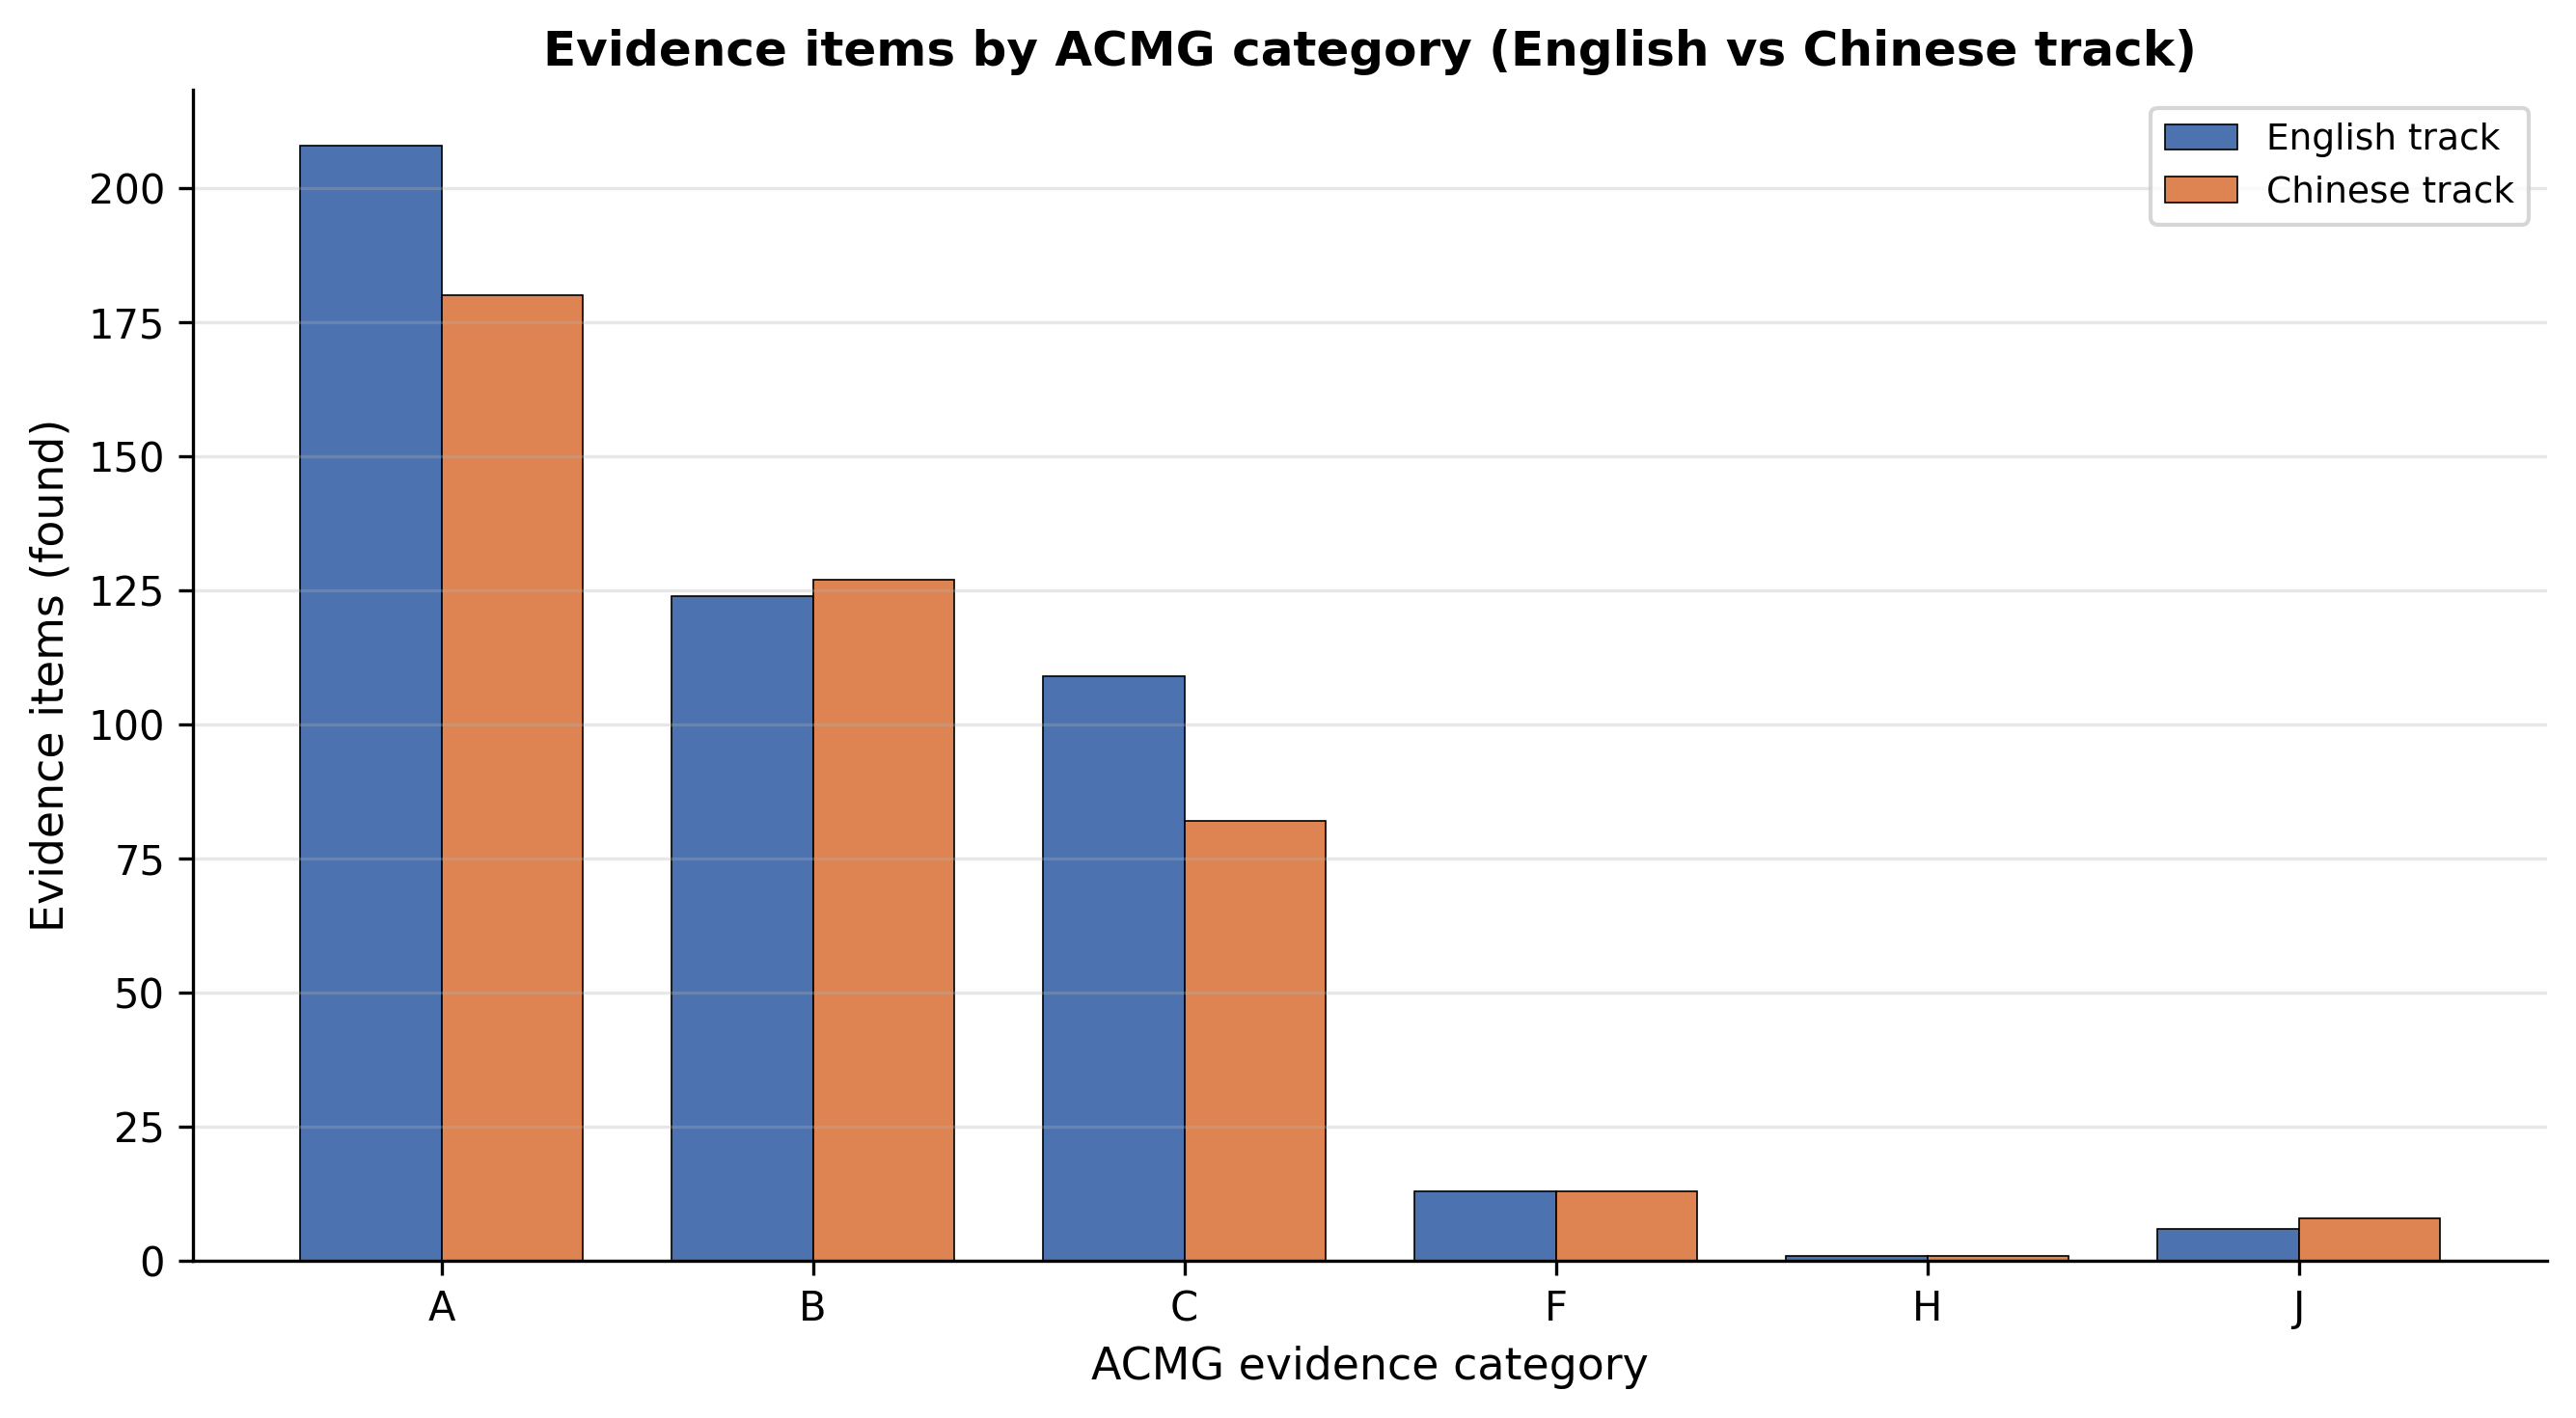
\includegraphics[width=0.9\textwidth]{S1_evidence_by_category.png}
  \caption{Total found evidence items by ACMG evidence category (A--J)
  for the English vs.\ Chinese extraction track, summed across the 29
  valid dual-track runs. The Chinese track adds items across categories,
  most visibly in category B (disease/phenotype) and category A
  (variant). Generated by
  \texttt{benchmark/analysis/generate\_gim\_figures.py} (requires per-run
  pipeline outputs; available from the authors on request due to size).}
  \label{fig:s1}
\end{figure}

\clearpage

\section*{Supplementary Table S1: Per-Entry Field Match (EN-only vs
Dual-track)}
\addcontentsline{toc}{section}{Supplementary Table S1: Per-Entry Field
Match}

Gold-standard field matches (of 8) for the 30 fused ClinGen/ClinVar
entries. Source: \path{ablation_report.json}.

\begin{table}[htbp]
  \centering
  \caption{Per-entry field match, EN-only vs.\ dual-track.}
  \label{tab:s1}
  \small
  \begin{tabular}{@{}llcccl@{}}
    \toprule
    \textbf{Entry} & \textbf{Gene} & \textbf{EN} & \textbf{Dual} &
    $\boldsymbol{\Delta}$ & \textbf{Field changes (EN$\rightarrow$Dual)} \\
    \midrule
    fused\_000 & CFTR   & 4 & 4 & 0    & --- \\
    fused\_001 & ABCA4  & 6 & 6 & 0    & --- \\
    fused\_002 & ACADVL & 5 & 5 & 0    & --- \\
    fused\_003 & ACTA1  & 5 & 5 & 0    & --- \\
    fused\_004 & ACTA1  & 6 & 6 & 0    & --- \\
    fused\_005 & ADA    & 3 & 4 & $+1$ & +variant\_type (missense) \\
    fused\_006 & APC    & 5 & 5 & 0    & --- \\
    fused\_007 & ATM    & 1 & 1 & 0    & --- \\
    fused\_016 & DNM2   & 5 & 5 & 0    & +moi\_reported,
      $-$gene\_disease\_rel (swap) \\
    fused\_022 & GJB2   & 4 & 3 & $-1$ & $-$disease\_diagnosis \\
    fused\_024 & GP1BA  & 0 & 1 & $+1$ & +gene\_symbol (GP1BA) \\
    fused\_028 & HBB    & 4 & 3 & $-1$ & $-$variant\_hgvs\_c \\
    \multicolumn{2}{@{}l}{\ldots\ (remaining 18 entries)} & = & = & 0 & --- \\
    \bottomrule
  \end{tabular}
\end{table}

\textbf{Summary:} mean 3.57/8 in both modes. 3/30 entries gained $\geq$1
field (fused\_005, fused\_016, fused\_024) and 3/30 lost $\geq$1 field
(fused\_016, fused\_022, fused\_028); fused\_016 both gained and lost one
field (swap). Net: 2 improved, 2 regressed, 26 unchanged. Per-field
discordance across 30 entries $\times$ 8 fields: $b = 3$ (dual-only
found), $c = 3$ (EN-only found), McNemar exact $p = 1.0$.

\clearpage

\section*{Supplementary Table S2: Field-Level Multilingual Benefit
(ZH-only Fields)}
\addcontentsline{toc}{section}{Supplementary Table S2: Field-Level
Multilingual Benefit}

Distribution of fields whose evidence was found only by the Chinese
track. Source: \path{multilingual_contribution_report.json} (29 valid
entries).

\begin{table}[htbp]
  \centering
  \caption{Fields with ZH-only evidence.}
  \label{tab:s2}
  \small
  \begin{tabular}{@{}llc@{}}
    \toprule
    \textbf{Field ID} & \textbf{Field} & \textbf{ZH-only entries} \\
    \midrule
    B.clinical\_phenotypes & Clinical phenotypes & 3 \\
    F.assay\_type & Assay type & 3 \\
    J.clinvar\_assertion & ClinVar assertion & 2 \\
    B.hpo\_terms & HPO terms & 2 \\
    B.age\_of\_onset & Age of onset & 2 \\
    B.disease\_diagnosis & Disease diagnosis & 2 \\
    C.de\_novo\_status & De novo status & 2 \\
    B.mode\_of\_inheritance\_reported & Mode of inheritance & 1 \\
    C.inheritance\_source & Inheritance source & 1 \\
    H.contradiction\_type & Contradiction type & 1 \\
    B.case\_count & Case count & 1 \\
    A.variant\_consequence\_class & Variant consequence class & 1 \\
    A.functional\_domain\_or\_hotspot & Functional domain / hotspot & 1 \\
    B.sex & Sex & 1 \\
    \bottomrule
  \end{tabular}
\end{table}

Total: 23 ZH-only field instances across 14 field types, distributed over
13/29 entries (44.8\%).

\clearpage

\section*{Supplementary Note S1: Literature Provider Coverage}
\addcontentsline{toc}{section}{Supplementary Note S1: Literature Provider
Coverage}

Providers integrated in Phase 1 (literature acquisition).

\begin{center}
  \small
  \begin{tabular}{@{}llll@{}}
    \toprule
    \textbf{Provider} & \textbf{Language/Region} & \textbf{Access} &
    \textbf{Notes} \\
    \midrule
    Crossref & International & REST API & DOI metadata \\
    PubMed & English & E-utilities & Core biomedical index \\
    OpenAlex & International & REST API & Open scholarly metadata \\
    EuropePMC & European & REST API & Open-access full text \\
    PMC & English & REST API & Full-text biomedical \\
    DOAJ & International & REST API & Open-access journals \\
    J-STAGE & Japanese & REST API & Japanese science \& technology \\
    Unpaywall & International & REST API & Open-access resolution \\
    CyberLeninka & Russian & Scraper & Russian academic literature \\
    Hans Publishers & Chinese & Scraper & Chinese open-access publisher \\
    PubScholar & Chinese & Scraper & Chinese public scholarship platform \\
    KoreaScience & Korean & Scraper & Korean science literature \\
    ChinaXiv & Chinese & Scraper & Chinese preprints \\
    Redalyc & Spanish/Portuguese & Scraper & Latin American journals \\
    arXiv/bioRxiv & English & REST API & Preprints \\
    \bottomrule
  \end{tabular}
\end{center}

\section*{Supplementary Note S2: ACMG Evidence Field Catalog (excerpt)}
\addcontentsline{toc}{section}{Supplementary Note S2: ACMG Evidence Field
Catalog}

Evidence fields extracted by the system, organized in categories
A--J. The eight gold-standard fields used for the field-match ablation
are marked (*).

\begin{center}
  \footnotesize
  \begin{tabular}{@{}p{5.6cm}p{3.8cm}p{4.2cm}l@{}}
    \toprule
    \textbf{Field ID} & \textbf{Field name} & \textbf{Description} &
    \textbf{Type} \\
    \midrule
    A.gene\_symbol* & Gene Symbol & HGNC gene symbol & text \\
    A.variant\_hgvs\_c* & Variant HGVS (c.) & cDNA-level nomenclature &
      text \\
    A.variant\_hgvs\_p* & Variant HGVS (p.) & Protein-level nomenclature &
      text \\
    A.variant\_type* & Variant Type & Variant class (missense, deletion,
      \ldots) & enum \\
    A.gene\_disease\_relationship* & Gene--Disease Relationship &
      Causative/associated/\ldots & enum \\
    B.disease\_diagnosis* & Disease Diagnosis & Reported diagnosis &
      text \\
    B.mode\_of\_inheritance\_reported* & Mode of Inheritance & AD/AR/XL/\ldots
      & enum \\
    J.clinvar\_assertion* & ClinVar Assertion & Clinical significance &
      enum \\
    B.clinical\_phenotypes & Clinical Phenotypes & Reported phenotypes &
      text \\
    B.hpo\_terms & HPO Terms & HPO-coded phenotypes & text \\
    B.age\_of\_onset & Age of Onset & Onset age & text \\
    C.de\_novo\_status & De Novo Status & Confirmed/assumed de novo &
      enum \\
    F.assay\_type & Assay Type & Functional assay class & text \\
    \multicolumn{4}{@{}l}{\ldots\ (full catalog in repository)} \\
    \bottomrule
  \end{tabular}
\end{center}

\section*{Supplementary Note S3: Translation Quality Validation}
\addcontentsline{toc}{section}{Supplementary Note S3: Translation Quality
Validation}

Multi-stage translation pipeline safeguards (implemented in
\path{backend/src/core/cross_lingual_translation/}):

\begin{enumerate}
  \item \textbf{Terminology preservation:} translation prompts constrain
    the handling of gene symbols, HGVS strings, and disease names;
    terminology echo artifacts are stripped in post-processing.
  \item \textbf{Structural alignment:} paragraph, table, and
    image-reference structure is preserved and validated between source
    and target.
  \item \textbf{Draft translation:} initial LLM translation pass with
    context-window management (whole-document or segmented mode).
  \item \textbf{Review \& refinement:} post-processing passes correct
    punctuation/placeholder normalization and strip
    prompt/source-contamination artifacts.
  \item \textbf{Validation:} deterministic checks verify translation
    completeness, per-block coverage, and target-language conformity, and
    flag redacted/missing values before the translated document enters
    extraction.
\end{enumerate}

\section*{Supplementary Note S4: Ablation Run Wall-Clock Durations}
\addcontentsline{toc}{section}{Supplementary Note S4: Ablation Run
Wall-Clock Durations}

Per-entry pipeline wall-clock durations recorded by the ablation runner
(\texttt{duration\_s} in
\path{en_only_metrics.json}\,/\,\path{dual_track_metrics.json}; $n = 30$
per mode). Runs executed against the live backend service under normal
operating load; durations therefore reflect deployment conditions rather
than a controlled latency benchmark.

\begin{center}
  \begin{tabular}{@{}lccc@{}}
    \toprule
    \textbf{Mode} & $\boldsymbol{n}$ & \textbf{Mean (s)} &
    \textbf{Median (s)} \\
    \midrule
    EN-only & 30 & 759.6 & 623.1 \\
    Dual-track (EN+ZH) & 30 & 612.6 & 416.5 \\
    \bottomrule
  \end{tabular}
\end{center}

The two modes were executed in separate batches at different times;
between-batch differences in backend load dominate the mode difference,
so these figures characterize practical throughput ($\sim$7--13 min per
entry end-to-end), not the marginal cost of the second track.

\section*{Supplementary Note S5: Comparison with Existing Tools}
\addcontentsline{toc}{section}{Supplementary Note S5: Comparison with
Existing Tools}

\begin{center}
  \small
  \begin{tabular}{@{}p{3.2cm}p{3.4cm}p{2.6cm}p{2.3cm}p{2.3cm}@{}}
    \toprule
    \textbf{Feature} & \textbf{Lingua Seeker} & \textbf{Mastermind} &
    \textbf{LitVar} & \textbf{ClinVar Miner} \\
    \midrule
    Literature language & Multilingual (7+) & English & English &
      English \\
    Retrieval & Semantic + keyword & Keyword & Keyword & Database query \\
    Full-text parsing & Yes (MinerU) & No & No & No \\
    Evidence extraction & LLM structured & Manual curation & Keyword
      matching & None \\
    Entity standardization & Yes (HGNC/OMIM/ HPO/ClinVar) & Partial &
      Partial & Yes \\
    ACMG field catalog & Yes & No & No & No \\
    Expert review loop & Yes (delta audit) & Yes & No & No \\
    Open source & Yes & No & No & No \\
    Web server & Yes & Yes & Yes & Yes \\
    \bottomrule
  \end{tabular}
\end{center}

\section*{Committed Data Files}
\addcontentsline{toc}{section}{Committed Data Files}

Located at \path{docs/gim/supplementary/reports/} in the repository.

\begin{center}
  \small
  \begin{tabular}{@{}lp{7.6cm}@{}}
    \toprule
    \textbf{File} & \textbf{Content} \\
    \midrule
    \path{ablation_report.json} & Field-match ablation, per-entry EN vs
      dual matches and field changes \\
    \path{multilingual_contribution_report.json} & Evidence-item yield,
      per-entry EN/ZH/combined counts and ZH-only fields \\
    \path{en_only_metrics.json} & Per-entry final-output metrics and
      durations, EN-only mode \\
    \path{dual_track_metrics.json} & Per-entry final-output metrics and
      durations, dual-track mode \\
    \path{ablation_summary.txt} & Plain-text run summary \\
    \bottomrule
  \end{tabular}
\end{center}

\end{document}
